\chapter{Concept Drift Detection}
\label{exp1}
\section{Data Used}

The whole dataset was collected by web crawler, containing 181903 fashion news in www.hypebeast.com from 20/04/2005 to 13/06/2018. A sample of the dataset including the date of the publication, the category, the keywords, the title, the context, the HYPES, and the class of the HYPES. The HYPES is the real time popularity metric informing reader of what is trending. The HYPES is computed based on the page-viewers, the comments, and the information flow on social network. The HYPES is classified into 3 classes which is shown in Table \ref{popularityclasses} of the introduction chapter. 

During the development of the website, HYPEBEAST also changed the algorithm of computing the HYPES. Figure \ref{hypes_yeas} shows the change of the HYPES from 2015 to 2018. And the distribution of each class over the past 13 years is presented in Figure \ref{proportion_yeas}. It is obvious that after the middle of 2013, HYPES have a significant jump and the present a rising trend until 2018. However, the proportions of classes remain stable after 2014. Based on this intuitive analysis, we select the data from 01/01/2014 to 13/08/2018 as the dataset for the experiment. It containing 95787 fashion news. The distribution of the classes is shown in Table \ref{distribution_classes}

\begin{figure}
\centering
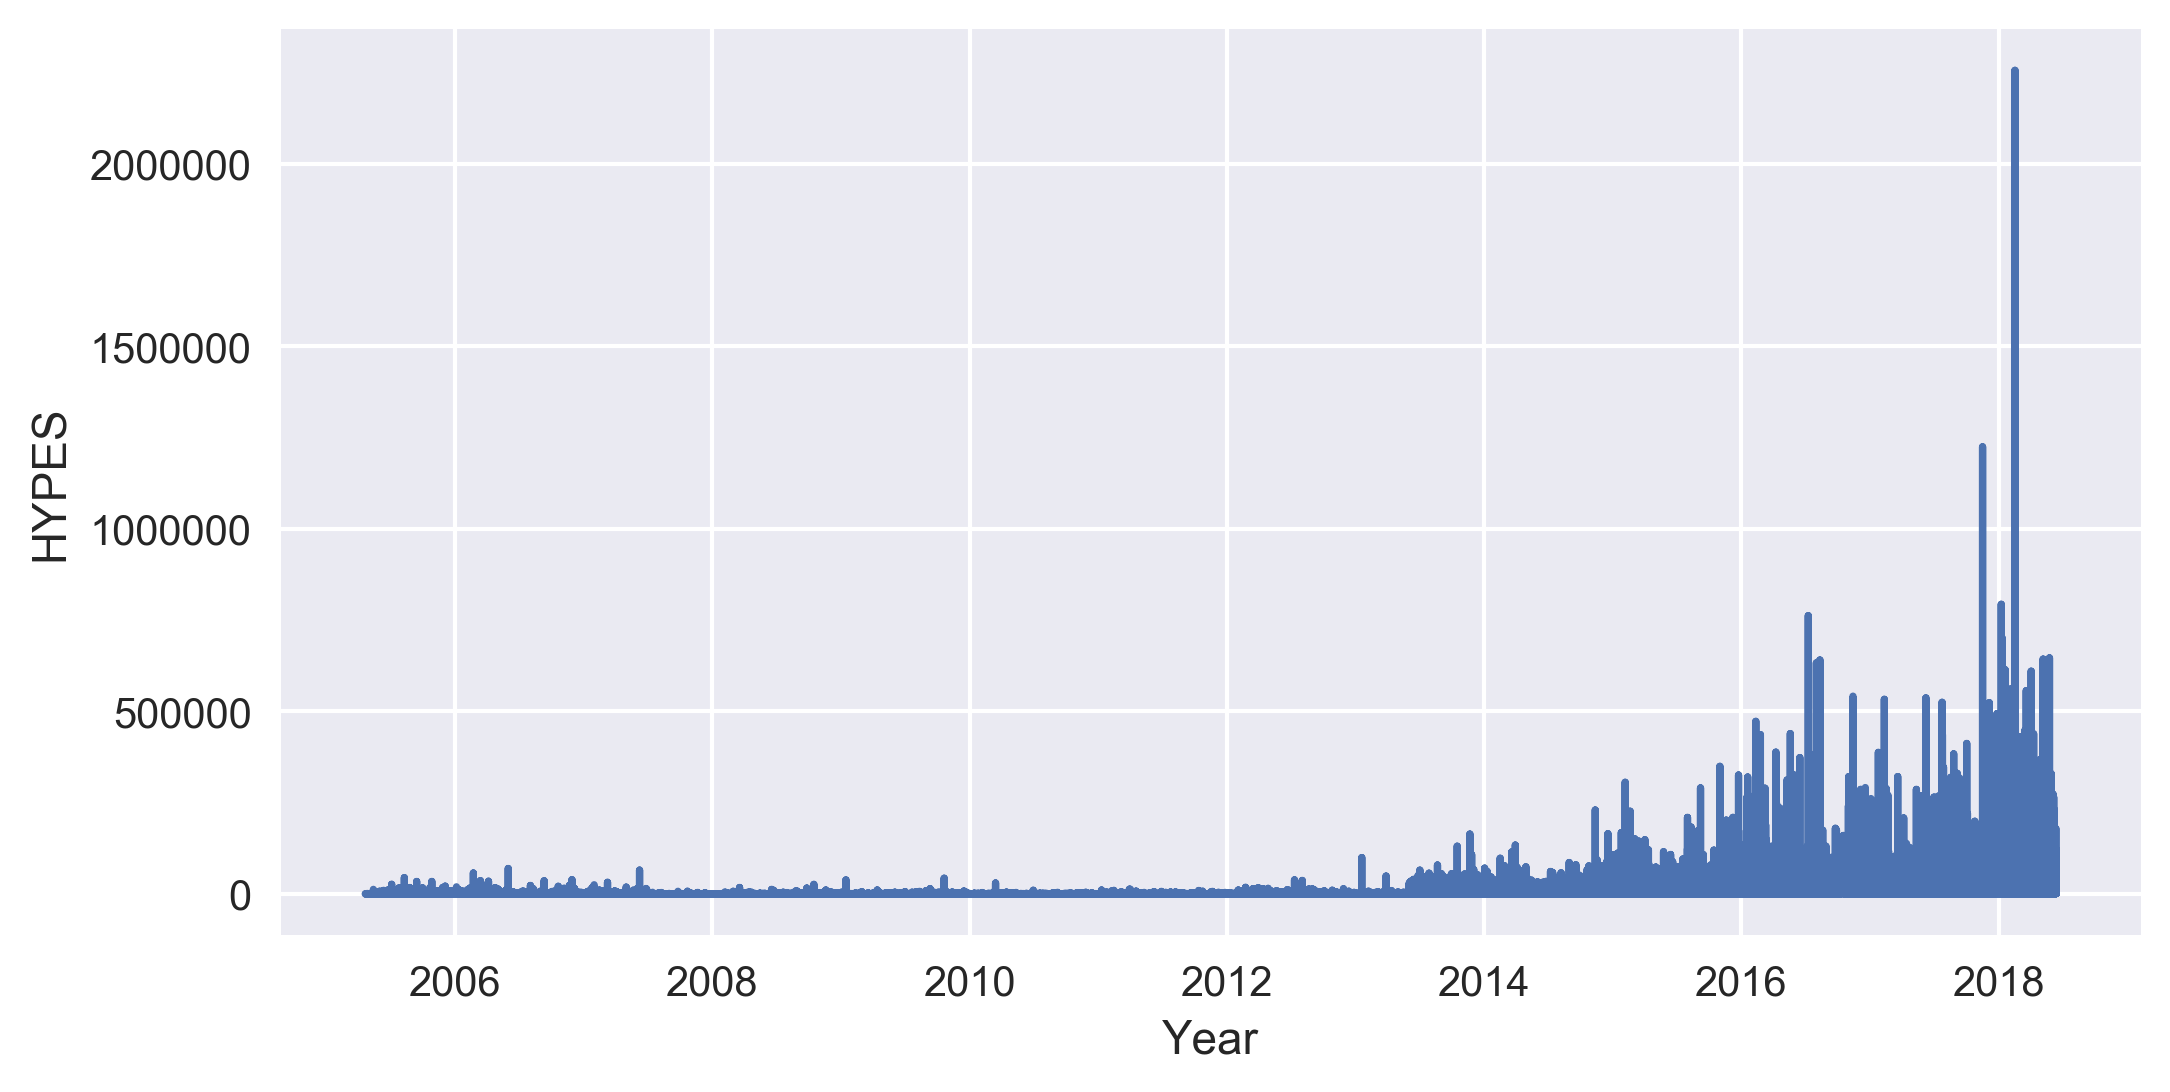
\includegraphics[width=0.9\textwidth]{hypes_year.png}
\caption{HYPES over years}
\label{hypes_yeas}

\end{figure}

\begin{figure}
\centering
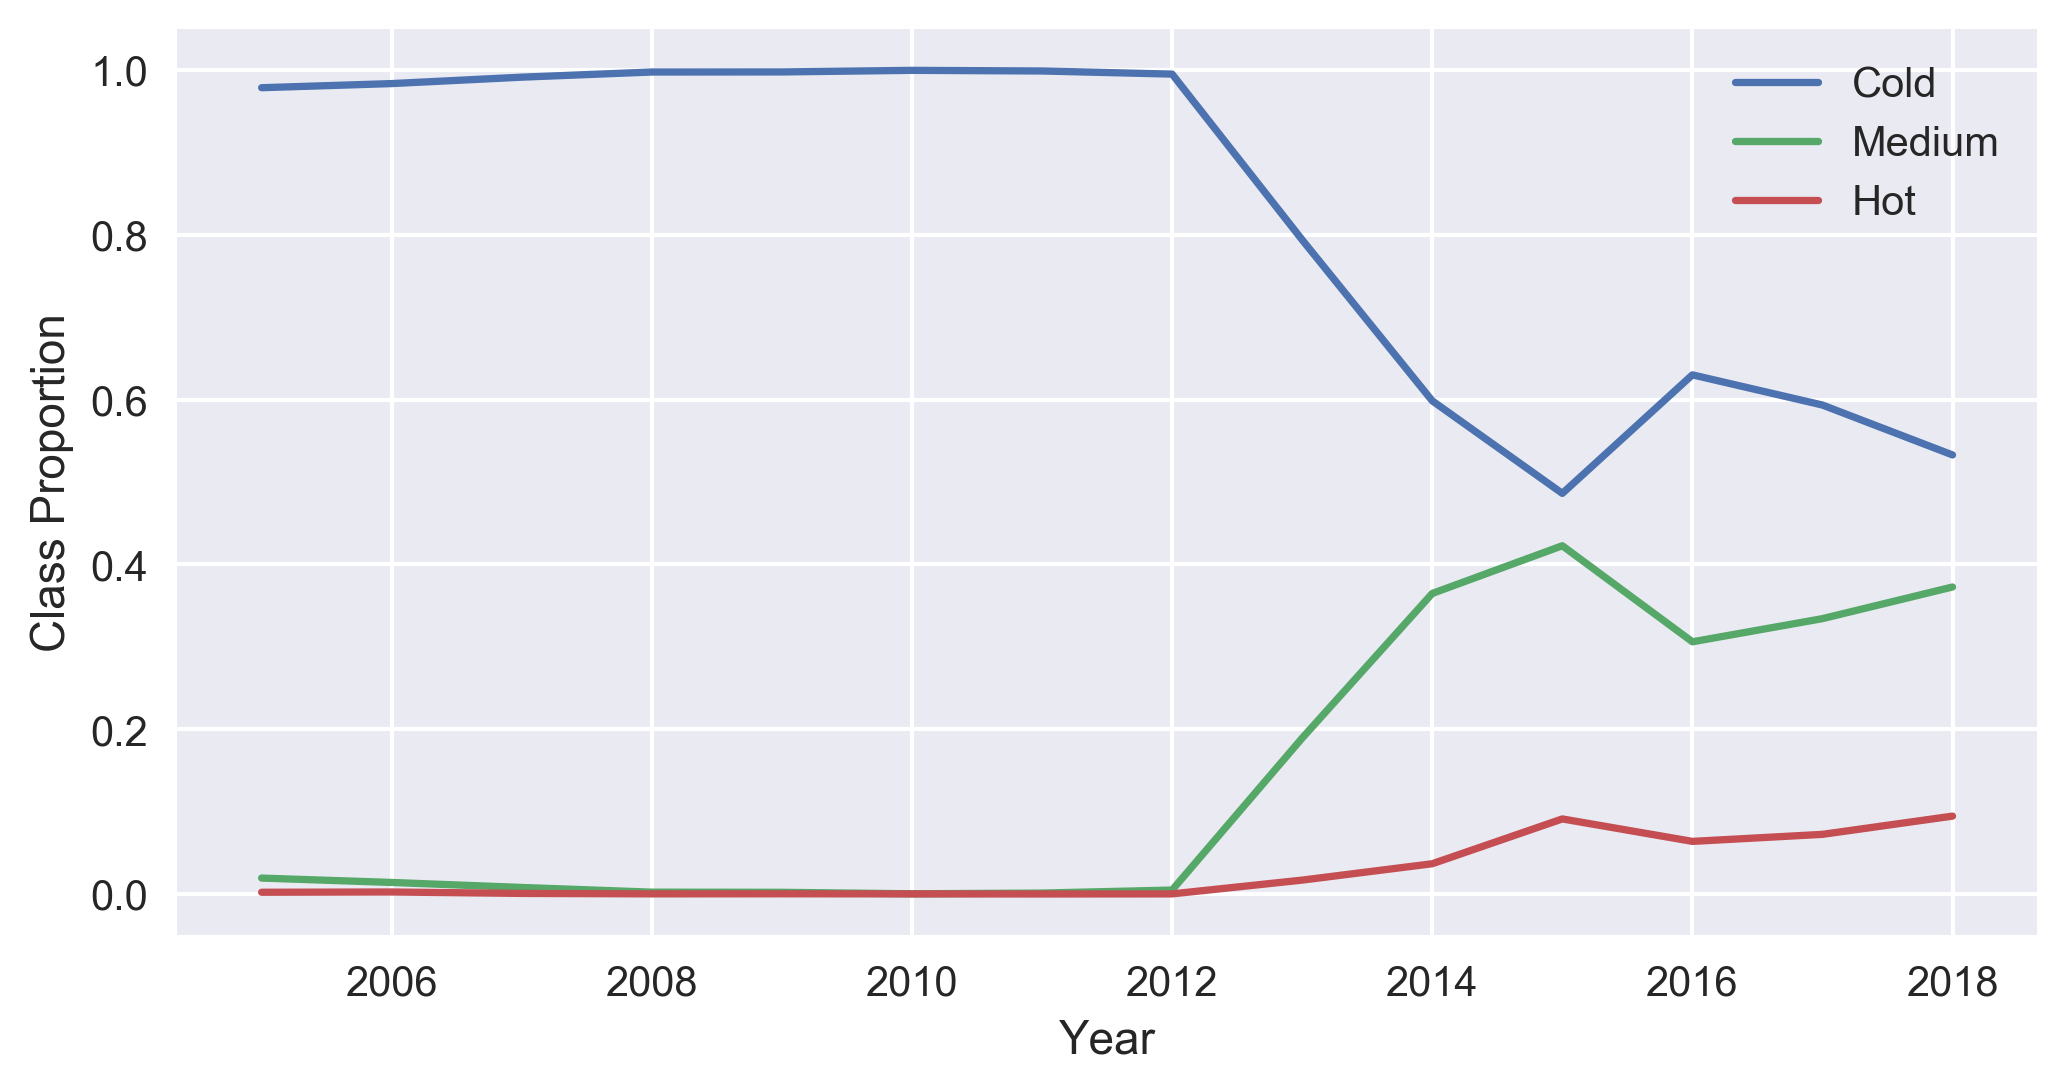
\includegraphics[width=0.9\textwidth]{proportion_hypes.png}
\caption{Proportion of each class over years}
\label{proportion_yeas}
\end{figure}


\begin{table}[]
\centering
\begin{tabular}{lll}
\multicolumn{1}{c}{Popularity} & \multicolumn{1}{c}{Number} & Proportion \\ \hline
Cold                           & 52852                      & 0.5518     \\
Meidum                         & 35944                      & 0.3752     \\
Hot                            & 6991                       & 0.0730    
\end{tabular}
\caption{Distribution of classes of the dataset}
\label{distribution_classes}
\end{table}




\section{Model Design}

\section{Result}